\clearpage
\Question{Spanning Trees}

\begin{parts}

\ifbool{practice}{\part}{\bonuspart[1]}%
\TAGS{spanning-tree}%
Consider the  25-vertex graph with 40 edges as shown below.

\begin{center}
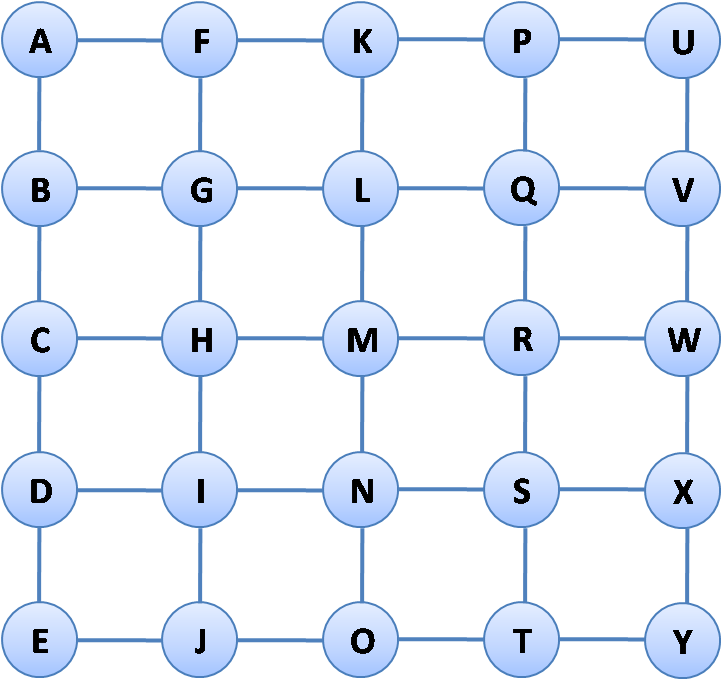
\includegraphics[width=0.5\linewidth]{\img/mazegraph.png}
\end{center}

Each vertex represents a room and each edge represents a door from one
room to another. We can form a maze from room A to room Y by computing
a spanning tree for this graph using a random permutation of the edge
set. Consider the edges in the order shown in the following random
permutation:

\begin{lstlisting}
  { HI, FK, PQ, KL, CH, ST, BG, RW, XY, EJ, KP, FG, DE, MN, IN,
    LM, PU, AB, SX, GL, GH, NO, DI, LQ, IJ, AF, QR, OT, WX, MR,
    RS, QV, CD, JO, HM, TY, UV, VW, NS, BC }
\end{lstlisting}

Starting with the graph below consisting of 25 disconnected
components, add an edge if and only if it connects two disconnected
components in the graph. Continue until all vertices are connected
into one component, i.e. a spanning tree.

\begin{framed}
\begin{center}
\ifprintanswers
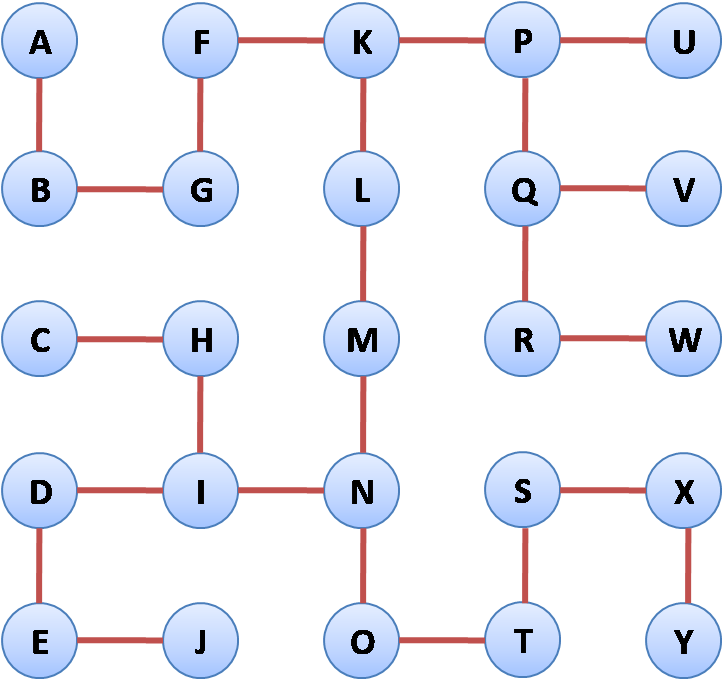
\includegraphics[width=0.9\linewidth]{\img/maze-spanning.png}
\else
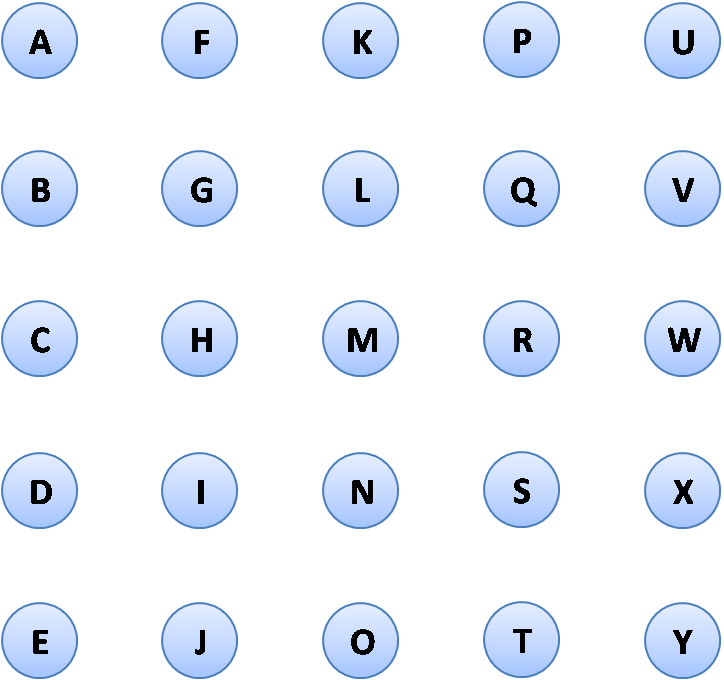
\includegraphics[width=0.9\linewidth]{\img/mazegraphnolines.png}
\fi
\end{center}
\smallskip
\end{framed}

\bigskip
How many edges from the random list were examined until you had a valid maze?

\bigskip
\begin{framed}
\medskip
\answer{34em}{32}
\end{framed}

\RUBRIC
Part (a)
TAGS: spanning-tree

Gradescope rubric:
+0.8pt  EITHER Correct graph
+0.4pt  OR     Up to 1 or 2 mistakes (like QV missing) or cycles
+0.2pt  correct number of edges (32 if graph is correct)

Commentary:
- Spanning tree:
  A  F--K--P--U
  |  |  |  |
  B--G  L  Q--V
        |  |
  C--H  M  R--W
     |  |
  D--I--N  S--X
  |     |  |  |
  E--J  O--T  Y
    (half a point for one or two mistakes/cycles, like QV missing)

- Number of edges:
  Full credit: 32 if the first graph is right (stop at QV)
  Full credit: 28 if first graph is missing QV (stop at OT)
  Full credit: 27 if they're missing edge QV and OT (stop at QR)
  Half credit for off-by-one.
  No credit for 24
ENDRUBRIC


\newpage
\ifbool{practice}{\part}{\bonuspart[1]}%
\TAGS{spanning-tree}%
Consider the following weighted graph with 9 vertices. Using Kruskal's
algorithm, list the edges that belong to the minimum spanning tree in
the order that they are added to the tree. Identify each edge by its
vertices as a two letter pair (e.g., $AB$) with the two vertices in
alphabetical order.  If there is a tie between edges to add to the
tree, choose the edge that comes first alphabetically. The first two
edges added to the minimum spanning tree are given for you.

\medskip
\begin{center}
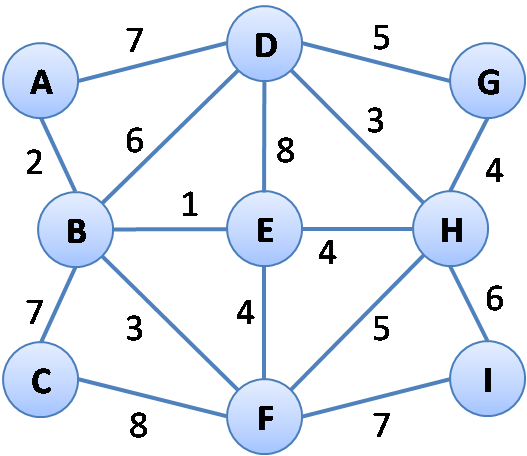
\includegraphics[width=0.4\textwidth]{\img/kruskals.png}
\end{center}

\medskip
\begin{framed}
\medskip
BE, AB, \answer{30em}{BF, \ DH, \ EH, \ GH, \ HI, \ BC}
\end{framed}

\RUBRIC
Part (b)
TAGS: spanning-tree

Gradescope rubric:
+1pt   EITHER: correct solution (BE, AB, BF, DH, EH, GH, HI, BC)
+0.5pt     OR: 1 or 2 errors

Commentary:
  BE, AB, BF, DH, EH, GH, HI, BC
    1/2 point for one or two errors
ENDRUBRIC

\bigskip
\ifbool{practice}{\part}{\bonuspart[1]}%
\TAGS{spanning-tree}%
Consider the following \emph{weighted} graph (whose edge weights not shown):

\begin{center}
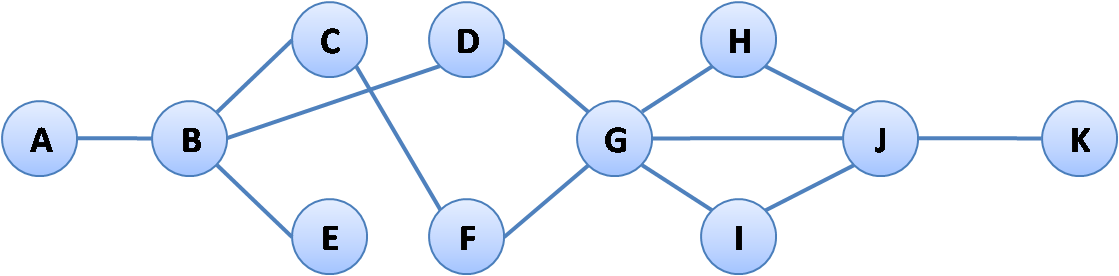
\includegraphics[width=0.85\textwidth]{\img/countmsts.png}
\end{center}

If all of the edge weights are unique, how many minimum spanning trees
does this graph have?

\medskip
\begin{framed}
\medskip
\answer{34em}{one}
\end{framed}

\medskip
If all of the edge weights are the same, how many minimum spanning
trees does this graph have?

\medskip
\begin{framed}
\medskip
\answer{34em}{1 * 1 * 5 * 8 * 1 = 40}
\end{framed}

\RUBRIC
Part (c)
TAGS: spanning-tree

Gradescope rubric:
+0.5pt  1st box: one
+0.5pt  2nd box: EITHER 5 * 8 = 40
+0.25pt 2nd box:     OR 35 or 45

Commentary:
* 2nd box:
  - Full credit: 5 * 8 = 40
  - 1pt for 35 or 45
ENDRUBRIC


% \newpage
% \part[1]\TAGS{complexity, spanning-tree}
% If a graph has $n$ vertices and is considered \emph{dense}, prove
% concisely why sorting the edges by weight using merge sort is
% $O(n^2$ log $n)$.

% \begin{framed}\bigskip\textbf{Solution: }
% \vspace{3in}
% \end{framed}

\end{parts}
